\documentclass[tikz,border=6pt]{standalone}
% shared TikZ style for the diagrams (colours match the plots)
\usepackage[T1]{fontenc}
\usepackage{lmodern}
\usepackage{amsmath,amssymb}
\usepackage{tikz}
\usetikzlibrary{arrows.meta,positioning,fit,backgrounds,calc,shapes.misc,decorations.pathreplacing}
\definecolor{cBlue}{HTML}{2A78D6}
\definecolor{cOrange}{HTML}{EB6834}
\definecolor{cAqua}{HTML}{1BAF7A}
\definecolor{cViolet}{HTML}{6250D6}
\definecolor{cGreen}{HTML}{008300}
\definecolor{cGray}{HTML}{8F8D86}
\definecolor{cInk}{HTML}{0B0B0B}
\definecolor{cInk2}{HTML}{52514E}
\tikzset{
  box/.style={draw=#1!70!black, fill=#1!10, rounded corners=3pt, align=center, inner sep=4pt, font=\small, line width=0.6pt},
  box/.default=cGray,
  arr/.style={-{Stealth[length=2.4mm]}, line width=0.8pt, cInk2},
  lbl/.style={font=\scriptsize, text=cInk2, align=center},
}

\begin{document}
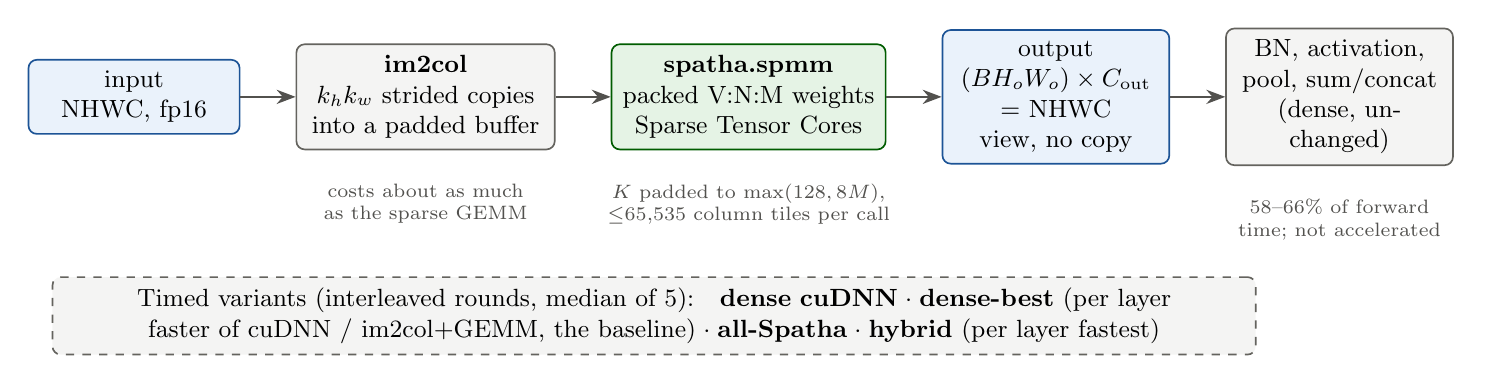
\begin{tikzpicture}[node distance=5mm and 7mm]
\node[box=cBlue, text width=24mm] (in) {input\\NHWC, fp16};
\node[box=cGray, text width=30mm, right=of in] (im) {\textbf{im2col}\\$k_hk_w$ strided copies\\into a padded buffer};
\node[box=cGreen, text width=32mm, right=of im] (sp) {\textbf{spatha.spmm}\\packed V:N:M weights\\Sparse Tensor Cores};
\node[box=cBlue, text width=26mm, right=of sp] (out) {output\\$(BH_oW_o)\times C_\text{out}$\\= NHWC view, no copy};
\node[box=cGray, text width=26mm, right=of out] (rest) {BN, activation,\\pool, sum/concat\\(dense, unchanged)};
\draw[arr] (in)--(im); \draw[arr] (im)--(sp); \draw[arr] (sp)--(out); \draw[arr] (out)--(rest);
\node[lbl, below=3mm of im, text width=34mm] {costs about as much\\as the sparse GEMM};
\node[lbl, below=3mm of sp, text width=36mm] {$K$ padded to $\max(128,8M)$,\\$\le$65{,}535 column tiles per call};
\node[lbl, below=3mm of rest, text width=32mm] {58--66\% of forward\\time; not accelerated};
\node[box=cGray, dashed, text width=150mm, below=16mm of sp, xshift=-12mm] (var) {Timed variants (interleaved rounds, median of 5):\quad \textbf{dense cuDNN}\;$\cdot$\;\textbf{dense-best} (per layer faster of cuDNN / im2col+GEMM, the baseline)\;$\cdot$\;\textbf{all-Spatha}\;$\cdot$\;\textbf{hybrid} (per layer fastest)};
\end{tikzpicture}
\end{document}
